\documentclass[12pt]{article}
\usepackage[utf8]{inputenc}
\usepackage{geometry}
\geometry{letterpaper, margin=0.25in}
\usepackage{graphicx} 
\usepackage{multicol}
\usepackage{parskip}
\usepackage{booktabs}
\usepackage{array} 
\usepackage{paralist} 
\usepackage{verbatim}
\usepackage{sectsty}
\usepackage[shortlabels]{enumitem}

\usepackage{amsmath}
\usepackage{amssymb}
\usepackage{mathtools}
\usepackage{empheq}
\usepackage{xcolor}
\usepackage{bbm}
\usepackage{tikz}
\usepackage{pgfplots}
\usepackage{tikz-cd}
\usepackage{circuitikz}
\usepackage{multirow}
\pgfplotsset{compat=1.18}
\usetikzlibrary{intersections, decorations.markings}
\tikzset{
    marking along/.style n args={2}{
        decoration={
                markings, 
                mark=at position #1 with {\arrow{#2}}
        },
        postaction={decorate}
        },
    marking along/.default={0.5}{>}
    wavy/.style={
        decorate,decoration={coil,aspect=0}
     },
    two marks/.style n args={1}{
        decoration={
            markings,
            mark=at position 0.25 with {\arrow{#1}},
            mark=at position 0.75 with {\arrow{#1}}
         },
         postaction={decorate}
    }
    two marks/.default={>}
}

\usepackage[numbered,framed]{matlab-prettifier}
\lstset{
  style              = Matlab-editor,
  basicstyle         = \renewcommand{\ttdefault}{zi4}\fontencoding{T1}\ttfamily\small, % Inconsolata, close to MATLAB's editor font
  numberstyle        = \fontencoding{T1}\fontfamily{zi4}\selectfont\scriptsize\color{gray},
  escapechar         = ",
  mlshowsectionrules = true,
}

\colorlet{mygreen}{green!50!teal}
\colorlet{darkblue}{blue!60!black}

\newcommand{\ans}[1]{\boxed{\text{#1}}}
\newcommand{\vecs}[1]{\langle #1\rangle}
\renewcommand{\hat}[1]{\widehat{#1}}

\renewcommand{\P}{\mathbb{P}}
\newcommand{\R}{\mathbb{R}}
\newcommand{\E}{\mathbb{E}}
\newcommand{\Z}{\mathbb{Z}}
\newcommand{\N}{\mathbb{N}}
\newcommand{\Q}{\mathbb{Q}}
\newcommand{\C}{\mathbb{C}}

\newcommand{\ind}{\mathbbm{1}}
\newcommand{\qed}{\quad \blacksquare}

\newcommand{\brak}[1]{\left\langle #1 \right\rangle}
\newcommand{\bra}[1]{\left\langle #1 \right\vert}
\newcommand{\ket}[1]{\left\vert #1 \right\rangle}

\newcommand{\abs}[1]{\left\vert #1 \right\vert}
\newcommand{\mfX}{\mathfrak{X}}
\newcommand{\ep}{\varepsilon}

\newcommand{\Ec}{\mathcal{E}}
\newcommand{\Nc}{\mathcal{N}}
\newcommand{\A}{\mathcal{A}}
\newcommand{\F}{\mathcal{F}}
\newcommand{\Cc}{\mathcal{C}}
\newcommand{\B}{\mathcal{B}}
\newcommand{\M}{\mathcal{M}}
\newcommand{\X}{\chi}
\renewcommand{\L}{\mathcal{L}}

\newcommand{\sub}{\subseteq}
\newcommand{\st}{\text{ s.t. }}
\newcommand{\card}{\text{card }}
\renewcommand{\div}{\vspace*{10pt}\hrule\vspace*{10pt}}
\newcommand{\surj}{\twoheadrightarrow}
\newcommand{\inj}{\hookrightarrow}
\newcommand{\biject}{\hookrightarrow \hspace{-8pt} \rightarrow}
\renewcommand{\bar}[1]{\overline{#1}}
\newcommand{\overcirc}[1]{\overset{\circ}{#1}}
\newcommand{\diam}{\text{diam }}
\newcommand{\iid}{\overset{	ext{iid}}{\sim}}

\renewcommand{\Re}{\text{Re}\,}
\renewcommand{\Im}{\text{Im}\,}
\newcommand{\Var}{\text{Var}\,}
\newcommand{\Cov}{\text{Cov}\,}
\renewcommand{\tt}[1]{\texttt{#1}}

\DeclareMathOperator*{\argmax}{\arg\max}
\DeclareMathOperator*{\argmin}{\arg\min}

\newcommand{\sign}{\text{sign}\,}

\newcommand*{\tbf}[1]{\ifmmode\mathbf{#1}\else\textbf{#1}\fi}

\usepackage{tcolorbox}
\tcbuselibrary{breakable, skins}
\tcbset{enhanced}
\newenvironment*{tbox}[2][gray]{
    \begin{tcolorbox}[
        parbox=false,
        colback=#1!5!white,
        colframe=#1!75!black,
        breakable,
        title={#2}
    ]}
    {\end{tcolorbox}}

\newenvironment*{exercise}[1][red]{
    \begin{tcolorbox}[
        parbox=false,
        colback=#1!5!white,
        colframe=#1!75!black,
        breakable
    ]}
    {\end{tcolorbox}}

\newenvironment*{proof}[1][blue]{
\begin{tcolorbox}[
    parbox=false,
    colback=#1!5!white,
    colframe=#1!75!black,
    breakable
]}
{\end{tcolorbox}}
\newenvironment*{proposition}[1][gray]{
    \begin{tcolorbox}[
        parbox=false,
        colback=#1!5!white,
        colframe=#1!75!black,
        breakable
    ]}
    {\end{tcolorbox}}


\usetikzlibrary{arrows.meta, calc}
\tikzset{
    blk/.style={draw, thick, minimum height=0.8cm, minimum width=1cm, inner sep=4pt},
    sumj/.style={draw, thick, circle, inner sep=0pt, minimum size=0.7cm},
    dot/.style={circle, fill, inner sep=0pt, minimum size=4pt},
    io/.style={circle, draw, fill=white, inner sep=0pt, minimum size=5pt},
    bd/.style={>=Stealth, thick, font=\small}
}

\begin{document}
\begin{multicols}{2}
    \begin{flushleft}
        \parbox{0.5\textwidth}{\Large ENGN 1931Y: Homework 2}
    \end{flushleft}
    \begin{flushright}
        \tbf{Milan Capoor}\\
         30 September 2026
    \end{flushright}
\end{multicols}
\div

\textbf{Note that the HW is 6 problems; final grade is out of 70.}

\section*{Problem 1 --- 10 points}
    For the following block diagram, called ``control canonical form'', calculate the transfer function for this system. Note that $a_i$ and $b_i$ are constants.

    \begin{center}
    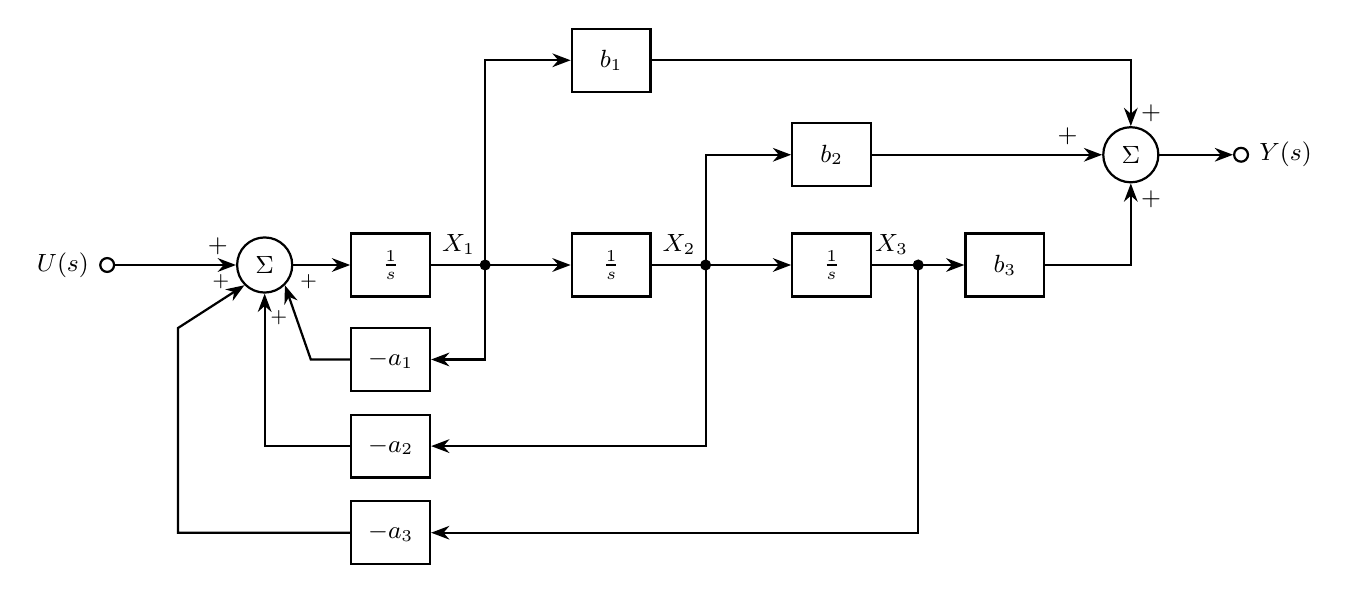
\begin{tikzpicture}[bd]
        \node[io, label=left:{$U(s)$}] (u) at (0,0) {};
        \node[sumj] (s1) at (2,0) {$\Sigma$};
        \node[blk] (i1) at (3.6,0) {$\frac{1}{s}$};
        \node[blk] (i2) at (6.4,0) {$\frac{1}{s}$};
        \node[blk] (i3) at (9.2,0) {$\frac{1}{s}$};
        \node[blk] (b3) at (11.4,0) {$b_3$};
        \node[sumj] (s2) at (13,1.4) {$\Sigma$};
        \node[io, label=right:{$Y(s)$}] (y) at (14.4,1.4) {};
        \node[blk] (b1) at (6.4,2.6) {$b_1$};
        \node[blk] (b2) at (9.2,1.4) {$b_2$};
        \node[blk] (a1) at (3.6,-1.2) {$-a_1$};
        \node[blk] (a2) at (3.6,-2.3) {$-a_2$};
        \node[blk] (a3) at (3.6,-3.4) {$-a_3$};

        \coordinate (x1) at (4.8,0);
        \coordinate (x2) at (7.6,0);
        \coordinate (x3) at (10.3,0);
        \node[dot] at (x1) {}; \node[dot] at (x2) {}; \node[dot] at (x3) {};

        \draw[->] (u) -- (s1) node[pos=0.85, above] {$+$};
        \draw[->] (s1) -- (i1);
        \draw[->] (i1) -- (i2);
        \draw[->] (i2) -- (i3);
        \draw[->] (i3) -- (b3);
        \node[above left] at (x1) {$X_1$};
        \node[above left] at (x2) {$X_2$};
        \node[above left] at (x3) {$X_3$};
        \draw[->] (b3) -| (s2) node[pos=0.9, right] {$+$};
        \draw[->] (b1) -| (s2) node[pos=0.9, right] {$+$};
        \draw[->] (b2) -- (s2) node[pos=0.85, above] {$+$};
        \draw[->] (s2) -- (y);

        \draw[->] (x1) |- (b1);
        \draw[->] (x2) |- (b2);
        \draw[->] (x1) |- (a1);
        \draw[->] (x2) |- (a2);
        \draw[->] (x3) |- (a3);
        \draw[->] (a1.west) -- ++(-0.5,0) -- (s1.south east);
        \draw[->] (a2) -| (s1);
        \draw[->] (a3) -| (0.9,-0.8) -- (s1.south west);
        \node[font=\scriptsize] at ($(s1.south east)+(0.3,0.05)$) {$+$};
        \node[font=\scriptsize] at ($(s1.south)+(0.18,-0.3)$) {$+$};
        \node[font=\scriptsize] at ($(s1.south west)+(-0.3,0.05)$) {$+$};
    \end{tikzpicture}
    \end{center}

    \color{darkblue}
        Let 
        \[T_1 = \frac{1/s}{1 + a_1/s}\]
        and 
        \[T_2 = \frac{T_1/s}{1 + T_1a_2/s}\]
        which reduces the system to 
        \begin{center}
        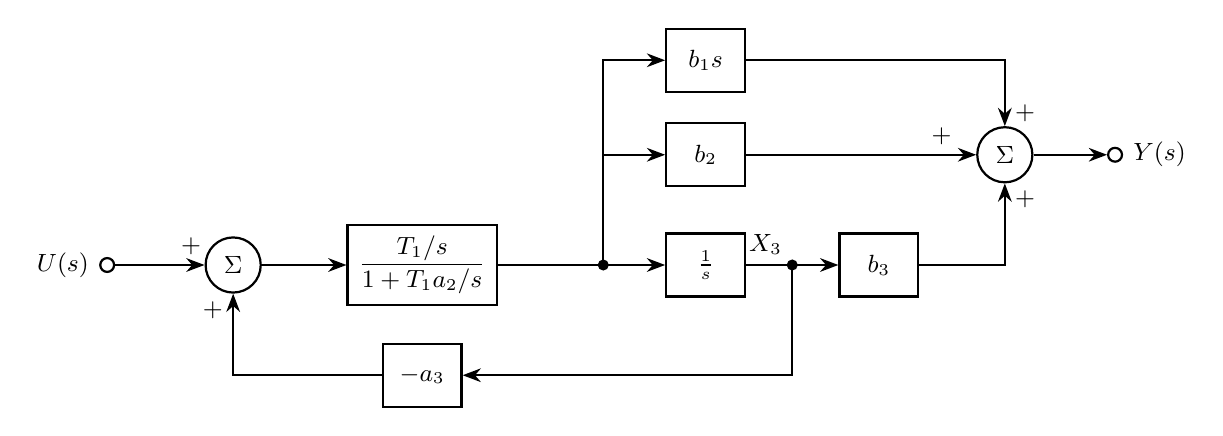
\begin{tikzpicture}[bd]
            \node[io, label=left:{$U(s)$}] (u) at (0,0) {};
            \node[sumj] (s1) at (1.6,0) {$\Sigma$};
            \node[blk] (x2b) at (4.0,0) {$\dfrac{T_1/s}{1 + T_1 a_2/s}$};
            \node[blk] (i3) at (7.6,0) {$\frac{1}{s}$};
            \node[blk] (b3) at (9.8,0) {$b_3$};
            \node[sumj] (s2) at (11.4,1.4) {$\Sigma$};
            \node[io, label=right:{$Y(s)$}] (y) at (12.8,1.4) {};
            \node[blk] (b1) at (7.6,2.6) {$b_1 s$};
            \node[blk] (b2) at (7.6,1.4) {$b_2$};
            \node[blk] (a3) at (4.0,-1.4) {$-a_3$};

            \coordinate (x2) at (6.3,0);
            \coordinate (x3) at (8.7,0);
            \node[dot] at (x2) {}; \node[dot] at (x3) {};

            \draw[->] (u) -- (s1) node[pos=0.85, above] {$+$};
            \draw[->] (s1) -- (x2b);
            \draw[->] (x2b) -- (i3);
            \draw[->] (i3) -- (b3);
            \node[above left] at (x3) {$X_3$};
            \draw[->] (b3) -| (s2) node[pos=0.9, right] {$+$};
            \draw[->] (b1) -| (s2) node[pos=0.9, right] {$+$};
            \draw[->] (b2) -- (s2) node[pos=0.85, above] {$+$};
            \draw[->] (s2) -- (y);

            \draw[->] (x2) |- (b1);
            \draw[->] (x2) |- (b2);
            \draw[->] (x3) |- (a3);
            \draw[->] (a3) -| (s1) node[pos=0.9, left] {$+$};
        \end{tikzpicture}
        \end{center}
        Now 
        \[T_3 = \frac{\frac{T_1/s}{s + T_1a_2}}{1 + \frac{a_3T_1/s}{s + T_1a_2}} = \frac{T_1}{s^2 + T_1(a_2s + a_3)}\]

        \begin{center}
        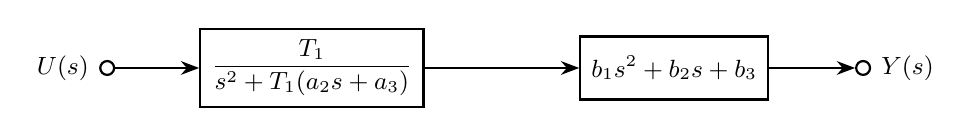
\begin{tikzpicture}[bd]
            \node[io, label=left:{$U(s)$}] (u) at (0,0) {};
            \node[blk] (x3b) at (2.6,0) {$\dfrac{T_1}{s^2 + T_1(a_2 s + a_3)}$};
            \node[blk] (b) at (7.2,0) {$b_1 s^2 + b_2 s + b_3$};
            \node[io, label=right:{$Y(s)$}] (y) at (9.6,0) {};

            \draw[->] (u) -- (x3b);
            \draw[->] (x3b) -- (b);
            \draw[->] (b) -- (y);
        \end{tikzpicture}
        \end{center}

        So 
        \begin{align*}
            \frac{Y(s)}{U(s)} &= \frac{T_1(b_1 s^2 + b_2 s + b_3)}{s^2 + T_1(a_2s + a_3)}\\ 
            &= \frac{\frac{1}{s + a_1}(b_1 s^2 + b_2 s + b_3)}{s^2 + \frac{1}{s + a_1}(a_2s + a_3)}\\ 
            &= \boxed{\frac{b_1 s^2 + b_2 s + b_3}{s^3 + a_1s^2 + a_2 s + a_3}}
        \end{align*}
    
    \color{black}


\section*{Problem 2 --- 15 points}
    For the following block diagrams, find the transfer function $Y/R$.

    \begin{center}
    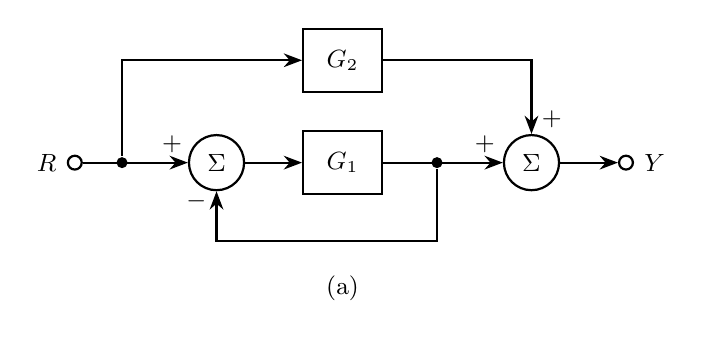
\begin{tikzpicture}[bd]
        \node[io, label=left:{$R$}] (r) at (0,0) {};
        \node[dot] (n0) at (0.6,0) {};
        \node[sumj] (s1) at (1.8,0) {$\Sigma$};
        \node[blk] (g1) at (3.4,0) {$G_1$};
        \node[dot] (n1) at (4.6,0) {};
        \node[sumj] (s2) at (5.8,0) {$\Sigma$};
        \node[io, label=right:{$Y$}] (y) at (7,0) {};
        \node[blk] (g2) at (3.4,1.3) {$G_2$};

        \draw[->] (r) -- (s1) node[pos=0.85, above] {$+$};
        \draw[->] (s1) -- (g1);
        \draw[->] (g1) -- (s2) node[pos=0.85, above] {$+$};
        \draw[->] (s2) -- (y);
        \draw[->] (n0) |- (g2);
        \draw[->] (g2) -| (s2) node[pos=0.9, right] {$+$};
        \draw[->] (n1) -- ++(0,-1) -| (s1) node[pos=0.9, left] {$-$};
        \node at (3.4,-1.6) {(a)};
    \end{tikzpicture}

    \color{darkblue}
        \begin{align*}
            T_1 &= \frac{G_1}{1 + G_1}\\ 
            \frac{Y}{R} &= T_1 + G_2 = \boxed{\frac{G_1 + G_2(1 + G_1)}{1 + G_1}}
        \end{align*}
    \color{black}

    \vspace{0.5cm}

    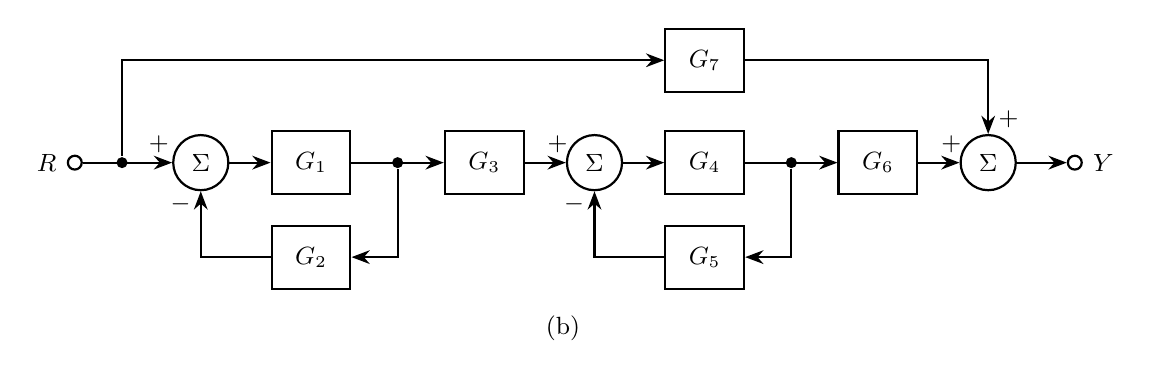
\begin{tikzpicture}[bd]
        \node[io, label=left:{$R$}] (r) at (0,0) {};
        \node[dot] (n0) at (0.6,0) {};
        \node[sumj] (s1) at (1.6,0) {$\Sigma$};
        \node[blk] (g1) at (3,0) {$G_1$};
        \node[dot] (n1) at (4.1,0) {};
        \node[blk] (g3) at (5.2,0) {$G_3$};
        \node[sumj] (s2) at (6.6,0) {$\Sigma$};
        \node[blk] (g4) at (8,0) {$G_4$};
        \node[dot] (n2) at (9.1,0) {};
        \node[blk] (g6) at (10.2,0) {$G_6$};
        \node[sumj] (s3) at (11.6,0) {$\Sigma$};
        \node[io, label=right:{$Y$}] (y) at (12.7,0) {};
        \node[blk] (g2) at (3,-1.2) {$G_2$};
        \node[blk] (g5) at (8,-1.2) {$G_5$};
        \node[blk] (g7) at (8,1.3) {$G_7$};

        \draw[->] (r) -- (s1) node[pos=0.85, above] {$+$};
        \draw[->] (s1) -- (g1);
        \draw[->] (g1) -- (g3);
        \draw[->] (g3) -- (s2) node[pos=0.8, above] {$+$};
        \draw[->] (s2) -- (g4);
        \draw[->] (g4) -- (g6);
        \draw[->] (g6) -- (s3) node[pos=0.8, above] {$+$};
        \draw[->] (s3) -- (y);
        \draw[->] (n1) |- (g2);
        \draw[->] (g2) -| (s1) node[pos=0.9, left] {$-$};
        \draw[->] (n2) |- (g5);
        \draw[->] (g5) -| (s2) node[pos=0.9, left] {$-$};
        \draw[->] (n0) |- (g7);
        \draw[->] (g7) -| (s3) node[pos=0.9, right] {$+$};
        \node at (6.2,-2.1) {(b)};
    \end{tikzpicture}

    \color{darkblue}
    
        \begin{align*}
            T_1 &= \frac{G_1}{1 + G_1 G_2}\\ 
            T_2 &= \frac{G_4}{1 + G_4 G_5}\\ 
            \frac{Y}{R} &= T_1 G_3 T_2 G_6 + G_7 = \boxed{\frac{G_1G_3G_4 G_6 + G_7(1 + G_1 G_2)(1 + G_4 G_5)}{(1 + G_1 G_2)(1 + G_4 G_5)}}
        \end{align*}
    \color{black}


    \vspace{0.5cm}

    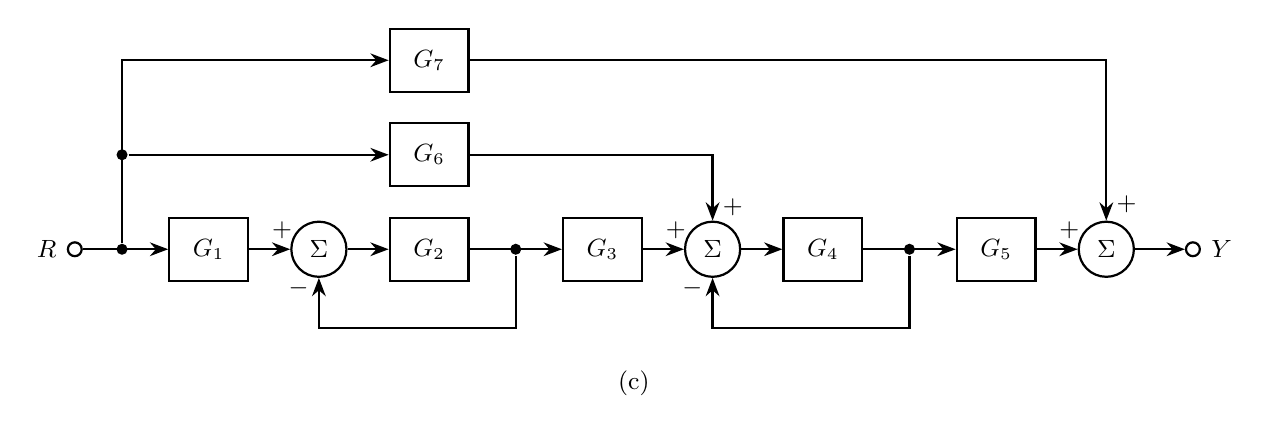
\begin{tikzpicture}[bd]
        \node[io, label=left:{$R$}] (r) at (0,0) {};
        \node[dot] (n0) at (0.6,0) {};
        \node[blk] (g1) at (1.7,0) {$G_1$};
        \node[sumj] (s1) at (3.1,0) {$\Sigma$};
        \node[blk] (g2) at (4.5,0) {$G_2$};
        \node[dot] (n1) at (5.6,0) {};
        \node[blk] (g3) at (6.7,0) {$G_3$};
        \node[sumj] (s2) at (8.1,0) {$\Sigma$};
        \node[blk] (g4) at (9.5,0) {$G_4$};
        \node[dot] (n2) at (10.6,0) {};
        \node[blk] (g5) at (11.7,0) {$G_5$};
        \node[sumj] (s3) at (13.1,0) {$\Sigma$};
        \node[io, label=right:{$Y$}] (y) at (14.2,0) {};
        \node[blk] (g6) at (4.5,1.2) {$G_6$};
        \node[blk] (g7) at (4.5,2.4) {$G_7$};
        \node[dot] (n3) at (0.6,1.2) {};

        \draw[->] (r) -- (g1);
        \draw[->] (g1) -- (s1) node[pos=0.8, above] {$+$};
        \draw[->] (s1) -- (g2);
        \draw[->] (g2) -- (g3);
        \draw[->] (g3) -- (s2) node[pos=0.8, above] {$+$};
        \draw[->] (s2) -- (g4);
        \draw[->] (g4) -- (g5);
        \draw[->] (g5) -- (s3) node[pos=0.8, above] {$+$};
        \draw[->] (s3) -- (y);
        \draw[->] (n1) -- ++(0,-1) -| (s1) node[pos=0.9, left] {$-$};
        \draw[->] (n2) -- ++(0,-1) -| (s2) node[pos=0.9, left] {$-$};
        \draw[->] (n0) |- (g7);
        \draw[->] (n3) -- (g6);
        \draw[->] (g6) -| (s2) node[pos=0.9, right] {$+$};
        \draw[->] (g7) -| (s3) node[pos=0.95, right] {$+$};
        \node at (7.1,-1.7) {(c)};
    \end{tikzpicture}

    \color{darkblue}
       \begin{align*}
         T_1 &= \frac{G_1G_2G_3}{1 + G_2} + G_6\\ 
         \frac{Y}{R} &= \frac{T_1G_4 G_5}{1 + G_4} + G_7\\ 
         &= \frac{\left(\frac{G_1G_2G_3}{1 + G_2} + G_6\right) G_4 G_5}{1 + G_4} + G_7\\ 
         &= \boxed{\frac{G_1 G_2 G_3G_4 G_5 + (1 + G_2)G_4 G_5 G_6 + (1+ G_2)(1 + G_4)G_7}{(1 + G_2)(1 + G_4)}}
        \end{align*}
    \color{black}
    \end{center}

\section*{Problem 3 --- 5 points}
    Use MATLAB to plot the step response for the following transfer function. Calculate the natural frequency and damping ratio using time-domain data. Use the \texttt{damp} command to verify.
    \[
        F(s) = \frac{2(s+3)}{(s+1)(s^2+6s+16)}
    \]

    \color{darkblue}
        \begin{lstlisting}[language=Matlab]
            s = tf('s');
            F = 2*(s + 3)/((s+1)*(s^2 + 6*s + 16))

            u = step(F);
            plot(u);

            [omega, zeta, poles] = damp(F);
        \end{lstlisting}
        produces
        \begin{center}
            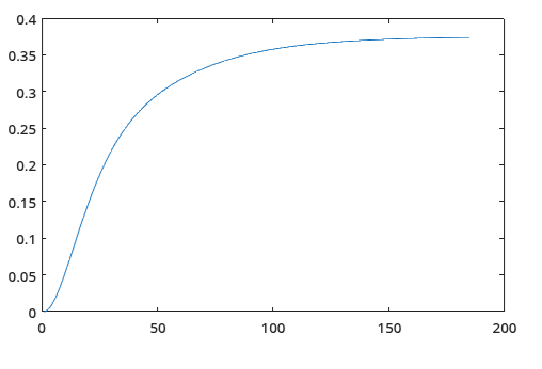
\includegraphics[width=0.5\textwidth]{Images/p3_step.png}
            \hspace{1in}
            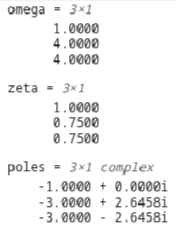
\includegraphics[width=0.2\textwidth]{Images/p3_poles.png}
        \end{center}

    \color{black}

\section*{Problem 4 --- 10 points}
    Derive the equations for a DC servo motor and show that the final equation is
    \[
        J_m \ddot{\theta}_m + \left(b + \frac{K_t K_e}{R_a}\right)\dot{\theta}_m = \frac{K_t}{R_a} v_a
    \]
    Assume that $J_m = 0.01\ \text{kg}\cdot\text{m}^2$, $b = 0.001\ \text{N}\cdot\text{m}\cdot\text{s}$, $K_e = 0.02\ \text{V}\cdot\text{s}$, $K_t = 0.02\ \text{N}\cdot\text{m/A}$, $R_a = 10\ \Omega$.
    \begin{enumerate}[(a)]
        \item Find the transfer function between the applied voltage and motor speed.
        \item What is the steady-state speed after a voltage $v_a = 10$ V has been applied?
        \item Find the transfer function between the applied voltage and shaft angle.
        \item Represent the above equation in state-space.
        \item Model the above equation in Simulink and find the steady-state velocity for applied voltages between 1 V and 10 V.
    \end{enumerate}

\section*{Problem 5 --- 10 points}
    For the unity feedback system shown below, use Simulink or MATLAB to design a proportional controller with gain $K$ that results in a maximum overshoot of 10\% in response to a unit step.

    \begin{center}
    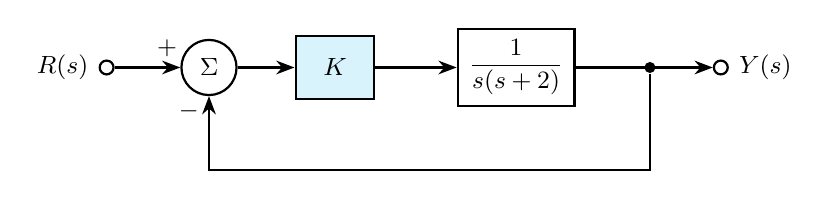
\begin{tikzpicture}[bd]
        \node[io, label=left:{$R(s)$}] (r) at (0,0) {};
        \node[sumj] (s1) at (1.3,0) {$\Sigma$};
        \node[blk, fill=cyan!15] (k) at (2.9,0) {$K$};
        \node[blk] (g) at (5.2,0) {$\dfrac{1}{s(s+2)}$};
        \node[dot] (n) at (6.9,0) {};
        \node[io, label=right:{$Y(s)$}] (y) at (7.8,0) {};

        \draw[->] (r) -- (s1) node[pos=0.8, above] {$+$};
        \draw[->] (s1) -- (k);
        \draw[->] (k) -- (g);
        \draw[->] (g) -- (y);
        \draw[->] (n) -- ++(0,-1.3) -| (s1) node[pos=0.9, left] {$-$};
    \end{tikzpicture}
    \end{center}

    \color{darkblue}
     Letting $k = 2.5$, 
    \begin{center}
        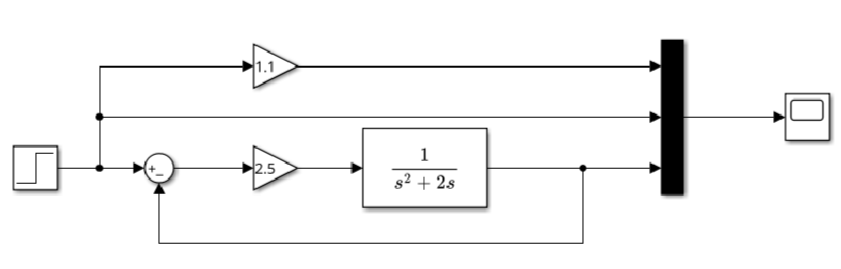
\includegraphics[width=0.8\textwidth]{Images/p5_simulink.png}
    \end{center}
    yields 
    \begin{center}
        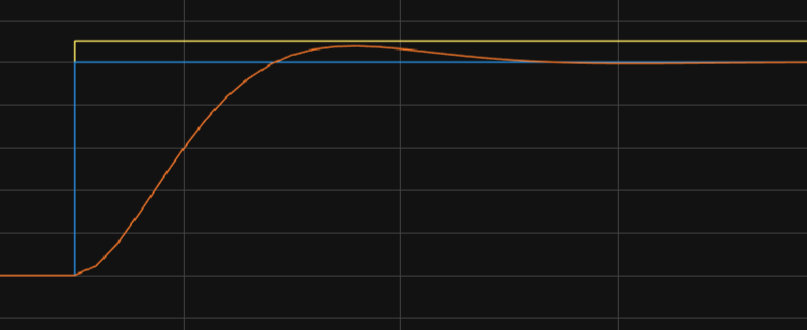
\includegraphics[width=0.8\textwidth]{Images/p5_graph.png}
    \end{center}
    \color{black}
   

\newpage
\section*{Problem 6 --- 20 points}
    The purpose of this problem is to design an analog compensator and perform MATLAB/Simulink simulation for position control of a DC motor as shown below:

    \begin{center}
    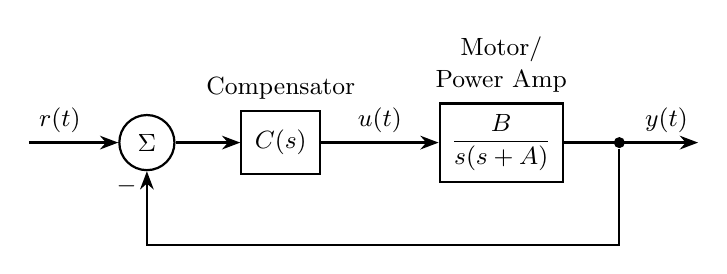
\begin{tikzpicture}[bd]
        \coordinate (r) at (0,0);
        \node[sumj] (s1) at (1.5,0) {$\Sigma$};
        \node[blk, label=above:{Compensator}] (c) at (3.2,0) {$C(s)$};
        \node[blk, label=above:{\shortstack{Motor/\\Power Amp}}] (p) at (6,0) {$\dfrac{B}{s(s+A)}$};
        \node[dot] (n) at (7.5,0) {};
        \coordinate (y) at (8.5,0);

        \draw[->] (r) -- (s1) node[pos=0, above right] {$r(t)$};
        \draw[->] (s1) -- (c);
        \draw[->] (c) -- (p) node[midway, above] {$u(t)$};
        \draw[->] (p) -- (y) node[pos=1, above left] {$y(t)$};
        \draw[->] (n) -- ++(0,-1.3) -| (s1) node[pos=0.9, left] {$-$};
    \end{tikzpicture}
    \end{center}

    where $A = 22$, $B = 120$. The inputs/outputs in the figure are defined as follows:
    \begin{itemize}
        \item $r(t)$: reference input in volts; 1 volt = 20 radians (a \underline{step} input of 1 volt)
        \item $y(t)$: motor position sensor output in volts (1 volt = 20 radians)
        \item $u(t)$: voltage input to plant
    \end{itemize}

    The design problem entails finding the values of the coefficients of the compensator $C(s)$, in the form
    \[
        C(s) = K \cdot \frac{s+a}{s+b},
    \]
    by iteration, while satisfying the following constraints:
    \begin{enumerate}[(a)]
        \item The maximum input to the motor should \underline{not} exceed $\pm 5$ V under any condition.
        \item Minimum rise time and settling time of the motor and \underline{no overshoot}.
    \end{enumerate}

    \textbf{Helpful procedure:}
    \begin{enumerate}[1.]
        \item Start with gain compensation $K$; choose the gain to give a critically damped response.
        \item Consider a first-order compensator $C(s)$ that gives a critically damped response.
        \item Consider the use of an input filter $F(s) = \dfrac{d}{s+d}$ that $r(t)$ goes through before reaching the summing junction. Design $d$, $a$, $b$, and $K$ to achieve the best settling time with no overshoot without violating the $\pm 5$ V constraint.
        \item Plot the results using MATLAB. Save the data to the workspace using either a scope or the ``To Workspace'' block.
        \item Use a transfer function block in MATLAB for the compensator:
\begin{verbatim}
>> numC = K*[1 a];
>> denC = [1 b];
\end{verbatim}
        Change the values of $K$, $a$, and $b$ from the workspace, and the Simulink diagram will change. Iterate the values of $a$ and $b$.
    \end{enumerate}
\end{document}